% IEEE Paper Template for A4 Page Size (V1)
% Sample Conference Paper using IEEE LaTeX style file for A4 pagesize.
% Copyright (C) 2006-2008 Causal Productions Pty Ltd.
% Permission is granted to distribute and revise this file provided that
% this header remains intact.
%
% REVISION HISTORY
% 20080211 changed some space characters in the title-author block
%
\documentclass[]{spie}
\usepackage{epsfig}
\usepackage{url}
\usepackage{multirow}
\usepackage{multicol}

\usepackage{amsmath}
\usepackage{amsfonts}
\usepackage{amssymb}
%\usepackage{amsthm}

\newcommand{\argmax}{\operatornamewithlimits{arg\,max}}

% paper title
\title{Heuristics for haplotype frequency estimation with a large number of analyzed loci}


\author{Micha\l{} Nowotka, Robert Nowak
  \skiplinehalf
  Faculty of Electronics and Information Technology\\
  Warsaw University of Technology\\
  Warsaw, Poland\\
}

\authorinfo{Further author information: (Send correspondence to Robert Nowak)\\
  Robert Nowak: E-mail: r.m.nowak@elka.pw.edu.pl}

\begin{document}
\maketitle

\begin{abstract}
Determining haplotypes with laboratory methods is an expensive and time-consuming
activity therefore unsuitable for the analysis of genetic data coming from a large number of tested
individuals. Many existing algorithms for phasing genotypes operate on very impractical runtime and
take into account only certain types of polymorphisms, often without providing graphical user interface.

The heuristic algorithm for estimating haplotype frequency developed in this work was
examined in terms of time complexity, the speed of execution and the accuracy of results. Consequently,
a Rich Internet Application that implements described algorithm has been created and its performance
and accuracy to a known set of test data is analyzed. Eventually, a discussion on the architecture and
the application’s usability in bioinformatics applications is presented.

Proposed algorithm can be used to improve the complexity of any algorithm that solves
the problem of genotype phasing, which has a worse time complexity and is convergent. The algorithm
is easy to scale and can achieve the desired ratio of calculations accuracy to execution time. Implemented
application meets all requirements for the programs to solve problems in biology i.e. high performance,
accessibility, scalability and usability.
\end{abstract}

\keywords{haplotype, locus, null allele, bioinformatics, genetics, heuristic, software system}

\section{Introduction}
In diploid organisms such as human there are two non-identical copies of autosomal chromosomes - one inherited from the mother, and another one from the father.
The combination of single nucleotide polymorphisms carried on the same chromosome is specific for each organism and called haplotype.
Although it is possible to directly determine haplotypes for a particular organism using laboratory techniques \cite{douglas},
such methods are very expensive and relatively slow.

\begin{figure}[!htb]
\centering
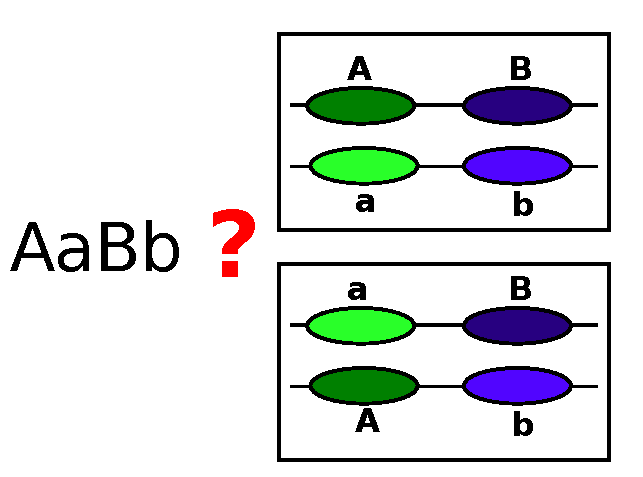
\includegraphics[scale=0.6]{images/poli}
\caption{The lack of phase information after typing leads to ambiguous of the haplotypes, example.}
\label{fig:poli}
\end{figure}

On the other hand, there are many effective techniques for determining unordered information about SNPs \cite{hapmap}.
This unstructured information is called genotype.
Genotypes provide information about alleles in loci but do not assign this information to chromosomes.

\begin{figure}[!htb]
\centering
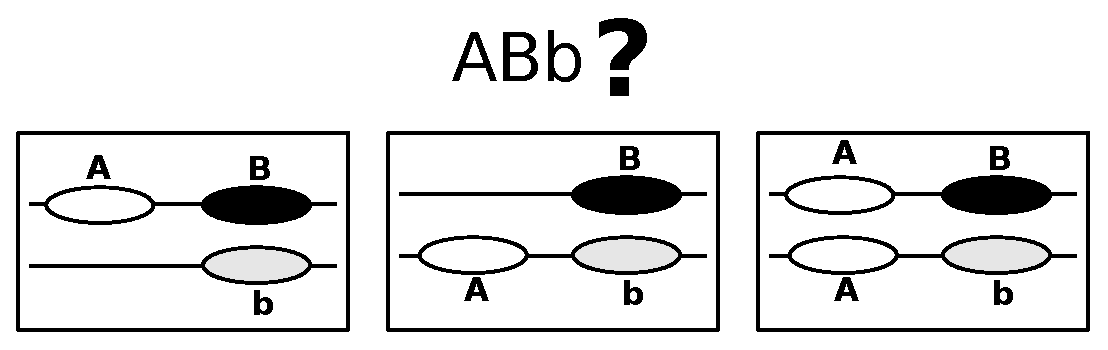
\includegraphics[scale=0.6]{images/null}
\caption{The ambiguous of the haplotypes for present-absent genes after typing, example.}
\label{fig:poli}
\end{figure}



In other words, if the genotype contains two different alleles for a specific locus,
there is no way to determine which of the alleles was inherited from the father and which from the mother, as depicted in Fig.~\ref{fig:poli}.
The problem is even more difficult if there are present-absent alleles (so called null alleles), as depicted in Fig.~\ref{fig:null}y.
Since haplotypes determine the exact sequence of the protein encoded by the genes,
finding it in human populations is an important step in identifying the genetic basis of complex diseases.
For this reason, algorithmic haplotype inference drawns the attention of many researchers.
The search space grows exponentially with number of considered loci,
if $Q$ is a set of haplotypes for given genotype, $h$ is number of observed heterozygous in this genotype, $n$ is number of observed (not null) alleles,
for loci having null allele,
$|Q| = 2^{h - 1}*3^{n}$ if we observe at least one heterozygous ($h > 0$) or $|Q|=\frac{3^{n}+1}{2}$ otherwise.
The large space is the main limitation of current used algorithms \cite{arlequin, phase, haploihp, nowak}.

\section{The algorithm}

In 2010 the computer program called NullHap was created at WUT \cite{nowak}.
The goal of the application was to estimate the probability of occurrences of haplotypes for a given population based on genotype observations.
The distinguishing feature of the application was the ability to operate on all possible types of loci -- both biallelic SNPs, as well as multiallelic loci or even null alleles.
One of the major drawbacks of the program is its exponential time complexity versus number of loci.
A recently published study \cite{gusev} suggests the possibility of substantial improvements in the complexity of the algorithm by introducing the concept of short overlapping window.

In the new approach a long genotype sequence would be divided into many short pieces of constant length, called windows, as depicted in Fig.~\ref{fig:window}.
The end of one window would be the beginning of a neighboring one.
The algorithm used by NullHap would not be applied to the whole genotype but just for windows and the results for a given window will be taken into account only when the beginning of a solution is compatible with the end solution of the previous window.
This solution should improve time complexity from exponential to linear.

\begin{figure}[!htb]
\centering
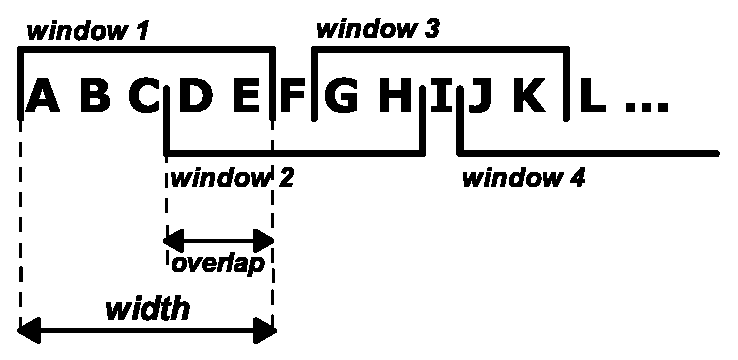
\includegraphics[scale=0.7]{images/window}
\caption{The window idea - sequence is divided into shorter, overlapping sub-sequence of constant length.}
\label{fig:window}
\end{figure}


The project aims to use this new approach for haplotype inference and compare with the NullHap program in terms of execution time and accuracy of results.
The end result will be to provide researchers a tool to estimate the haplotype frequencies that is efficient, scalable, portable and provide user friendly interface.

EM (Expectation-Maximization) algorithm \cite{em}  is used in statistics for finding maximum likelihood estimates of parameters in the probabilistic model when the model depends on the hidden variables that cannot be directly observed.
EM is an iterative algorithm that performs the Expectation step, that calculates the expected probability value for the current distribution of hidden variables, and the Maximization step, which calculates the value of the parameters that maximize the probability found in the E step.
These parameters are then used to determine the distribution of hidden variables in the next E step.
EM belongs to local optimization algorithms, which means that it can be trapped in local extreme.
It converges, that is, not moving away from the optimal solution over time.

The estimation of haplotypes probability to maximise the probability of observed sample
can be described by the equation given below, where $h_{i}$ are haplotypes, $G$ is number of observed genotypes,
$S = (n_{1}, n_{2},\ldots{},n_{G})$ is observed sample, $|Q_{j}|$ is number of elements in set of haplotypes for genotype $j$.

\begin{eqnarray*}
  \argmax_{h_{1}, h_{2}, ..., h_{H}} P( S~| h_{1}, h_{2}, ..., h_{H} ) =
  \argmax_{h_{1}, h_{2}, ..., h_{H}} \prod_{j=1}^{G}(\sum_{i=0}^{|Q_{j}|}z_{mn})^{n_{j}},
  \\
  ~z_{mn} =
  \left\{
  \begin{array}{ll}
    h_{m}^2          & \mbox{for}~m = n~\\
    2~h_{m} h_{n}    & \mbox{for}~m \not = n
  \end{array}
  \right.
  \nonumber
  \label{eqZadanie}
\end{eqnarray*}

Application of EM algorithm to inferring haplotypes has exponential time complexity.

Due to the unsatisfactory time complexity of the EM algorithm, it has been wrapped in a higher-level algorithm that uses a property of convergence of the EM.
In the first step genotype is divided into smaller fragments called windows.
Window properties are determined by width and overlap parameters.
For each window most probable haplotypes are computed.
Next, the partial haplotypes are combined.
This is done by the following rule: two neighbouring haplotypes can be combined if and only if all alleles at the common loci are the same.
The program generates all possible combinations of haplotype connections and evaluates each of them.
Then the resulting haplotypes are ordered by decreasing values of evaluation function.
The more windows overlap with each other, the less combinations need to be evaluated.
Reducing the amount is the purpose of overlapping windows.

\section{The architecture}

Implemented application is a kind of RIA (Rich Internet Application) based on the client-server model.

\begin{figure}[!htb]
\centering
\includegraphics{images/scheme2}
\caption{Application architecture - main modules.}
\label{fig:scheme}
\end{figure}

For the end user (most often a biologist) this means that all the functionality can be accessed from a web browser using very intuitive graphical user interface.
The sample window is depicted in Fig.~\ref{fig:organisms}.
That also means the application can be run on different hardware and software architectures.
The server side part can be installed on every Linux box using a few standard commands.
No additional software is needed.
Configuration is stored in a handful of human readable configuration files already containing reasonable settings.
All this is done to speed up deployment process and improve user experience.

\begin{figure}[!htb]
\centering
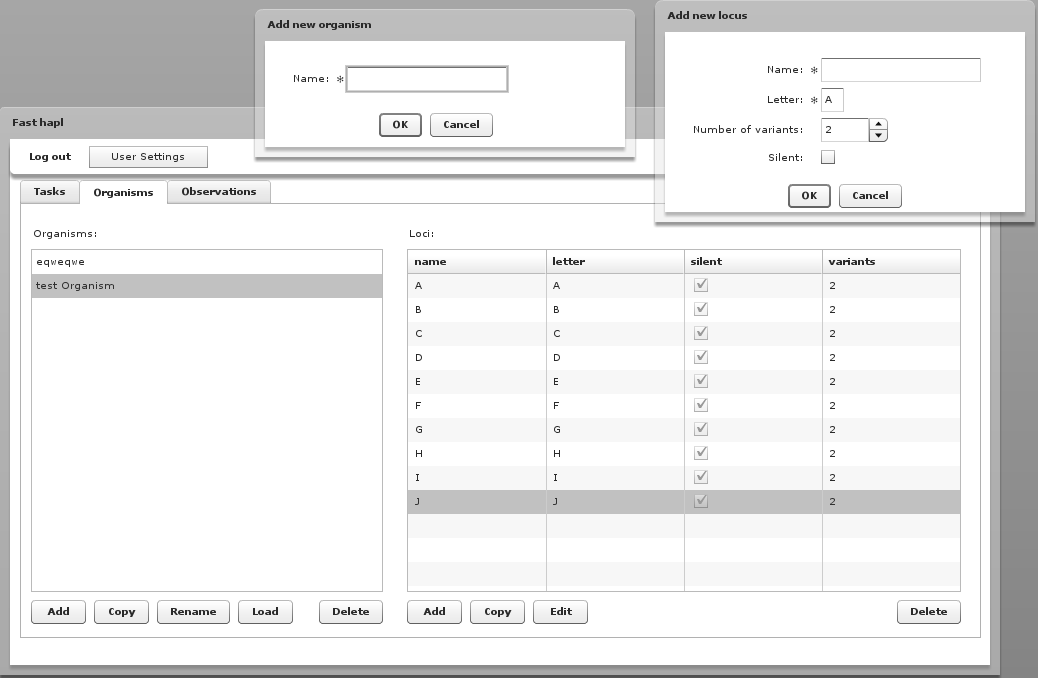
\includegraphics[scale=0.4]{images/Organisms}
\caption{Application window for defining the loci, alleles and organisms.}
\label{fig:organisms}
\end{figure}

Logically the application is spitted into three layers, as depicted in Fig.~\ref{fig:scheme}.
Presentation layer, located on the client side in a secure environment of web browser sandbox is implemented in ActionScript language using Flex framework.

Data (persistency) layer is implemented on the client side using Python language and Django object-relational mapping.
This makes it easier to switch between many data models -- which is especially important in early stages of development,
different database engines can also be changed easily.

Application layer is implemented in C++ and Python.
The usage of fast C++ language is aimed at eliminating bottlenecks in the most time-critical part of the application.
Modular design makes the application very flexible and generic \cite{boost}.
Any part can be replaced with another implementation and possibly improve the results.

\section{Results}

Test data consisted of well-known genotype set.
All genotypes contained null alleles and had 10 loci each.
It describes polymorphic killer inhibitory receptor (KIR) genes for genotyping 90 unrelated blood donors and 52 individuals from 13 families
\cite{crum2000development}.
Solving the problem of size 10 is time-consuming for a PC computer and the time can be measured easily.
The presence of null alleles makes full use of the algorithm.
In addition, for such a length one can choose a wide variety of width and overlap parameters.

\begin{figure}[!htb]
\centering
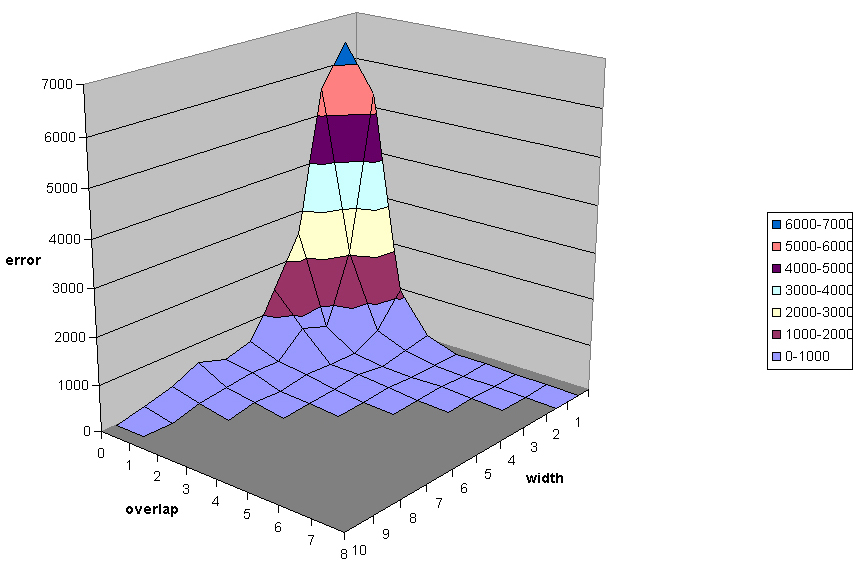
\includegraphics[scale=0.4]{images/error}
\caption{Error as a function of width and overlap parameters}
\label{fig:error}
\end{figure}

\begin{figure}
\centering
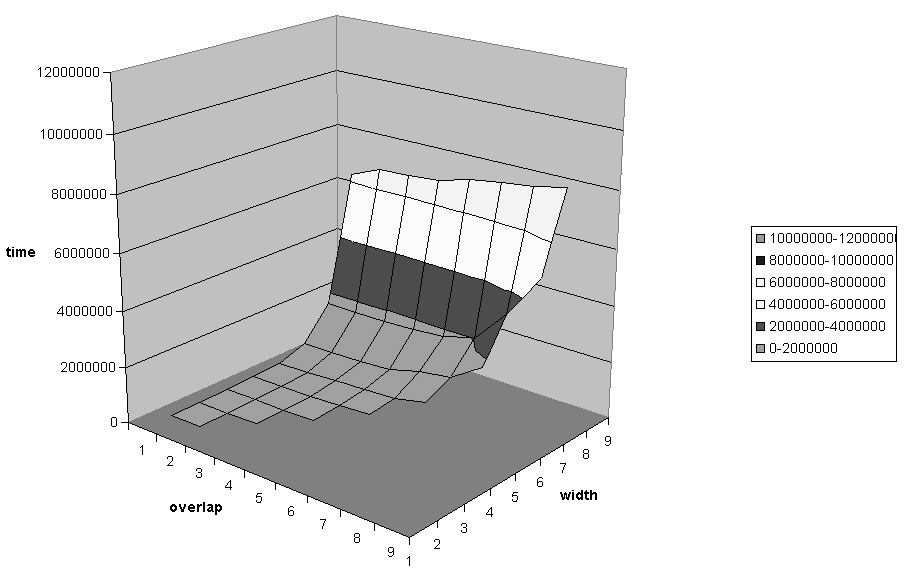
\includegraphics[scale=0.4]{images/czas}
\caption{Execution time as a function of width and overlap parameters}
\label{fig:time}
\end{figure}


The measurements were performed for every possible combination of width and overlap parameters.
For each combination the experiment was repeated five times and results along with averaged time were recorded.
All measurements were performed on a computer with an Intel Core Duo T9550 (2.66 GHz), 2GB of RAM.

Error function is the sum of the absolute values of the difference between a rank position of haplotype given by the windowless version and the rank position of the same haplotype produced by algorithm using windows.
$$ Error = \sum_{k=1}^{hap} |R^{*}(k) - R(k)|$$

The results are presented in two surface charts.
One of them illustrates the error as a function of width and overlap parameters.
Note the similarity of the graph to the graph presented in \cite{gusev}.
The second one shows the execution time in milliseconds.
There is an exponential relationship between the error function and the parameters of the window.
On the other hand, execution time increases linearly with overlap parameter and exponential with window length.


\section{Conclusions}

Results show that new approach scales very well.
There is wide variety of different combinations of with and overlap parameters where the error is negligible.
Only in the corner cases error value grows rapidly.
What is more, increasing overlap improves accuracy exponentially but time is increases only linearly which laverates and scales computation.

\bibliographystyle{spiebib}
\bibliography{hap2}

\end{document}
